\documentclass[12pt, oneside]{scrartcl}
	
% For figures
\usepackage{graphicx}
\graphicspath{{./figures/}} % specify relative path with extra {}

% Gets rid of section numbers
\renewcommand*{\sectionformat}{}

% No indentation throughout file
\setlength\parindent{0pt}

% Remove page numbers
\pagestyle{empty}

% formatting the captions of figures
\usepackage[bf]{caption} % make headings boldfont

% for drawing :-)
\usepackage{tikz} 
\usetikzlibrary{backgrounds} % to have a background layer
\usepackage{xcolor} % defining my own colors
\usetikzlibrary{positioning} % arrows between nodes and relative positions
\usetikzlibrary{arrows}


% Define colors
\colorlet{sampleShade}{gray!40}  % shading of sample trials
\colorlet{choiceShade}{blue!40}  % shading of choice trials
\colorlet{choiceCol}{red!70} % color of chosen option



% Some variables for drawing
\newcommand\sideAdj{13}
\newcommand{\imgSize}{.2\textwidth}
\newcommand{\descrTextWidth}{4cm}

\begin{document}

\section{Welcome to the experiment!}

We are interested in how humans make value based decisions and how these decisions are neurophysiologically grounded in the brain. The focus of this current study lies on a particular framework called \textit{Decisions from experience} as illustrated by the following scenario.

\begin{quotation}
\noindent Before purchasing a new laptop, a consumer may look for information on the relative merits of various available models such as online reviews, prices, or technical specifications. We call this search for information a “sequential sampling” of the available options. At some point, a consumer must stop the search for information and choose one laptop model, often without having obtained full certainty about which model is the best.
\end{quotation}


Our main interest for the present study are the neural mechanisms that underlie the sequential allocation of active sampling efforts to the choice options in question. Furthermore, we are interested in how humans arrive at a decision to terminate their information search. \\

To study these mechanisms, we have devised a set of paradigms in which you have agreed to participate today. These paradigms represent the scenario described above in simple terms. You will always have to decide between two options that both represent a lottery. Each of these lotteries will have a probability to yield either a winning outcome or a losing outcome. However, these probabilities are unknown and have to be learned through sampling. \\


\begin{figure}[h!]
\begin{center}
\resizebox{.9\linewidth}{!}{%
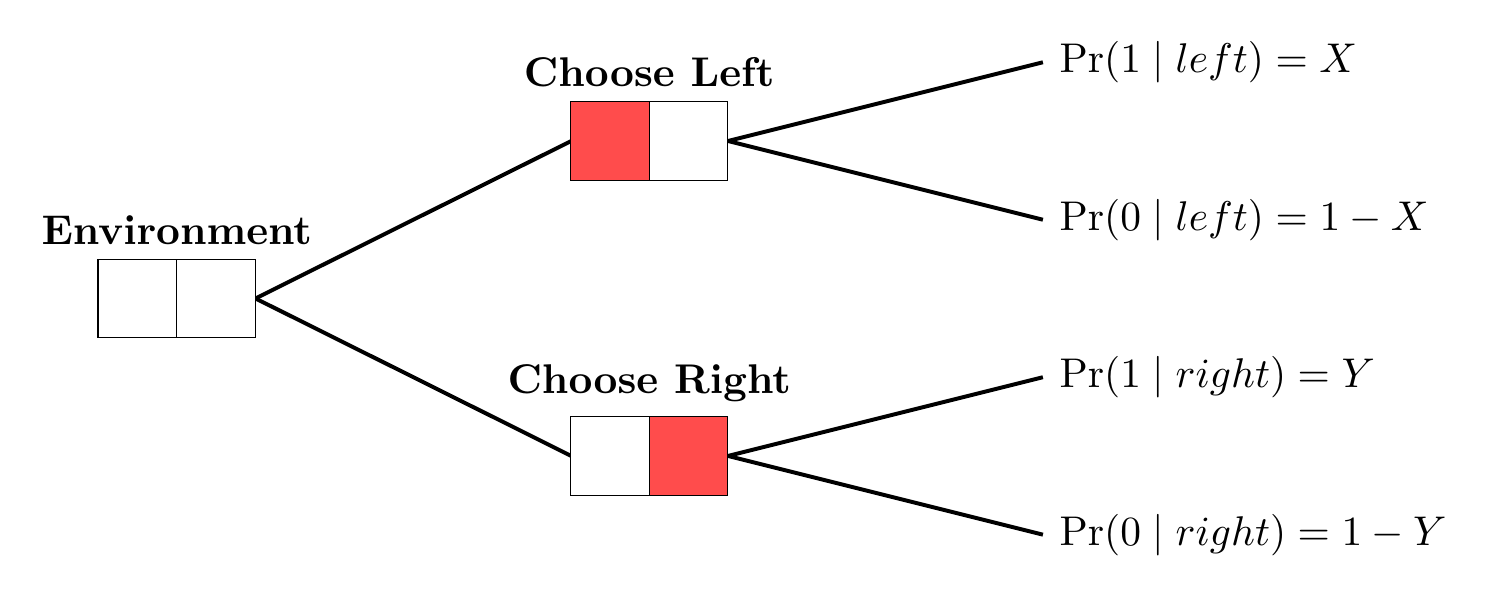
\begin{tikzpicture}
%--------------------------------------------------

% drawing two initial rectangles as environment
\filldraw [color=black, fill=white](4,15) rectangle (5,16)node[above, scale=1.5]{\textbf{Environment}};
\filldraw [color=black, fill=white](5,15) rectangle (6,16);


% now "left choice" rectangles
\filldraw [color=black, fill=choiceCol](10,17) rectangle (11,18)node[above, scale=1.5]{\textbf{Choose Left}};
\filldraw [color=black, fill=white](11,17) rectangle (12,18);


% now "right choice" rectangles
\filldraw [color=black, fill=white](10,13) rectangle (11,14) node[above, scale=1.5]{\textbf{Choose Right}};
\filldraw [color=black, fill=choiceCol](11,13) rectangle (12,14);



\begin{scope}[on background layer]
% Drawing lines to the choice rectangles
\draw [line width=0.5mm](6,15.5) -- (10.01,17.5);
\draw [line width=0.5mm](6,15.5) -- (10.01,13.5);

% Drawing lines to outcome probabilities 
\draw [line width=0.5mm](12,13.5) -- (16,14.5) node[right, scale=1.5]{$\Pr({1 \mid right})=Y$};
\draw [line width=0.5mm](12,13.5) -- (16,12.5)node[right, scale=1.5]{$\Pr({0 \mid right})=1-Y$};

\draw [line width=0.5mm](12,17.5) -- (16,18.5)node[right, scale=1.5]{$\Pr({1 \mid left})=X$};
\draw [line width=0.5mm](12,17.5) -- (16,16.5)node[right, scale=1.5]{$\Pr({0 \mid left})=1-X$};

\end{scope}

%--------------------------------------------------
\end{tikzpicture}
} % closing bracket from scaling
\captionsetup{width=.9\linewidth, format=plain}
\caption[Binary Lottery]{A binary lottery. $X$ and $Y$ refer to some probabilities.}
\label{fig:binLot}
\end{center}
\end{figure}


Although all tasks follow this general principle, there will be small differences between them. We will describe each of the tasks in more detail right before it starts. Furthermore, you will always be allowed to practice the task before you start. If you have questions at any point, do not hesitate to ask the experimenter.








\pagebreak
\section{Bandit}

This task consists out of a structure, where we have separate \textit{games}, in which a fixed number of \textit{trials} are nested. For each trial, you must choose between two options [left] and [right]. These options represent binary lotteries, which have a certain probability to yield a winning outcome and a certain probability to yield a losing outcome. Your task is, to maximize the winning outcomes for each game that you play. This is most easily done by exploring the options a bit, and learning their underlying probabilities to yield winning or losing outcomes. However, it is important to realize that each outcome that you see contributes to your payoff.  \\

Thus, it is a good strategy to try to balance exploration of the options and exploiting the knowledge you have already gained about the options. \\

You don’t know the probabilities of the lotteries in advance, but you do know that during one game with a fixed number of trials, the probabilities of the lotteries and their locations [left] and [right] remain stable. Once all trials within one game have been completed, the lotteries are shuffled and a new game is started.

At the end of the overall experiment, we will calculate the percentage of winning outcomes to all outcomes and multiply it with a monetary amount, that you can earn in Euros additionally to your show up fee.





\pagebreak
\section{Bandit Replay}

This task is very similar to the task you have just performed. However, instead of choosing between options and learning their underlying probabilities to yield winning or losing outcomes, you are watching a replay. Your task is to fixate upon the fixation cross and experience the replay of the previous task. Importantly, there will be one addition: Occasionally, a known outcome will be replaced by a distractor outcome. As soon as you realize that such a distractor trial has happened, you have to press the [space] button. \\

At the end of the overall experiment, we will calculate your reaction time to the distractor trials. From all of these reaction times, we will calculate the percentage that were below a certain time threshold and we will multiply it with a monetary amount that you can earn in Euros additionally to your show up fee. \\


\begin{figure}[h!]
\begin{center}
\includegraphics[scale=0.3]{distr_left.jpg}
\caption{An outcome during a distractor trial.}
\label{distr_left}
\end{center}
\end{figure}



\pagebreak
\section{Sampling Paradigm}

This task consists out of a structure, where we have separate \textit{games}, in which \textit{trials} are nested. For each trial, you can choose between two options [left] and [right]. These options represent binary lotteries, which have a certain probability to yield a winning outcome and a certain probability to yield a losing outcome. \\

However, you can also choose to not sample one of the options [left] or [right] and instead press [down]. When you press [down], you get to a stage of the game, where you must decide, which of the options [left] or [right] you find preferable. Then, an outcome will be generated from the option that you preferred. Your task is to maximize the winning outcomes that are obtained from this last game stage, after pressing [down]. \\

Thus, the structure of the task is separated into two parts: During the first part, you can freely sample the options [left] and [right] to learn their underlying probabilities to yield winning or losing outcomes. After learning the options to a sufficient degree, you can exploit your knowledge of the options and press [down]. This will bring you to the stage of the game, where you can decide for one lottery over the other and draw your outcome that counts towards your payoff. \\

At the end of the overall experiment, we will calculate the percentage of winning outcomes in the final stage to all outcomes in the final stage and multiply it with a monetary amount, that you can earn in Euros additionally to your show up fee.





\pagebreak
\section{Sampling Paradigm Replay}

This task consists out of a structure, where we have separate \textit{games}, in which \textit{trials} are nested. For each trial, you can choose between two options [left] and [right]. These options represent binary lotteries, which have a certain probability to yield a winning outcome and a certain probability to yield a losing outcome. \\

However, you can also choose to not sample one of the options [left] or [right] and instead press [down]. When you press [down], you get to a stage of the game, where you must decide, which of the options [left] or [right] you find preferable. Then, an outcome will be generated from the option that you preferred. Your task is to maximize the winning outcomes that are obtained from this last game stage, after pressing [down]. \\

Thus, the structure of the task is separated into two parts: During the first part, you can freely sample the options [left] and [right] to learn their underlying probabilities to yield winning or losing outcomes. After learning the options to a sufficient degree, you can exploit your knowledge of the options and press [down]. This will bring you to the stage of the game, where you can decide for one lottery over the other and draw your outcome that counts towards your payoff. \\

At the end of the overall experiment, we will calculate the percentage of winning outcomes in the final stage to all outcomes in the final stage and multiply it with a monetary amount, that you can earn in Euros additionally to your show up fee. \\

\begin{figure}[h!]
\begin{center}
\includegraphics[scale=0.3]{distr_right.jpg}
\caption{An outcome during a distractor trial.}
\label{distr_right}
\end{center}
\end{figure}




\end{document}